% Standalone vector figure extracted from manuscript.tex.
% Rebuild all figures from the project root: bash tkz/build.sh
\documentclass[tikz,border=2pt,class=IEEEtran]{standalone}
\usepackage{amsmath,amssymb,amsfonts}
\usepackage{xcolor}
\usetikzlibrary{positioning,arrows.meta,calc,backgrounds}

% Match the manuscript's IEEE Access text and math font settings.
\renewcommand{\textbf}[1]{{\fontseries{b}\selectfont #1}}
\renewcommand{\textit}[1]{{\itshape #1}}
\makeatletter
\AtBeginDocument{%
  \fontencoding{T1}\rmfamily\fontseries{m}\fontsize{10}{12}\selectfont
  \gdef\operator@encoding{T1}%
  \gdef\encodingdefault{T1}}
\makeatother

% ---- shared palette for review figures ----
\definecolor{cVLA}{HTML}{34618E}   % VLA lane / policy blue
\definecolor{cWM}{HTML}{9E4A3F}    % world-model lane
\definecolor{cCONV}{HTML}{5E4B8B}  % convergence purple
\definecolor{cGood}{HTML}{3A7D44}  % verified green
\definecolor{cWarn}{HTML}{B07A2A}  % caution amber
\definecolor{cPale}{HTML}{F2F0EA}  % pale panel fill
\tikzset{
  fnode/.style={draw=black!55, fill=white, rounded corners=1.5pt,
                inner sep=2.5pt, align=center, font=\fontsize{8}{9.5}\selectfont},
  flane/.style={draw=none, rounded corners=2pt, inner sep=3pt,
                align=center, font=\fontsize{8}{9.5}\selectfont\bfseries, text=white},
  farr/.style={-{Stealth[length=2mm]}, thick, black!60},
}


\newcommand{\figfont}{\fontsize{8}{9.5}\selectfont}

\begin{document}

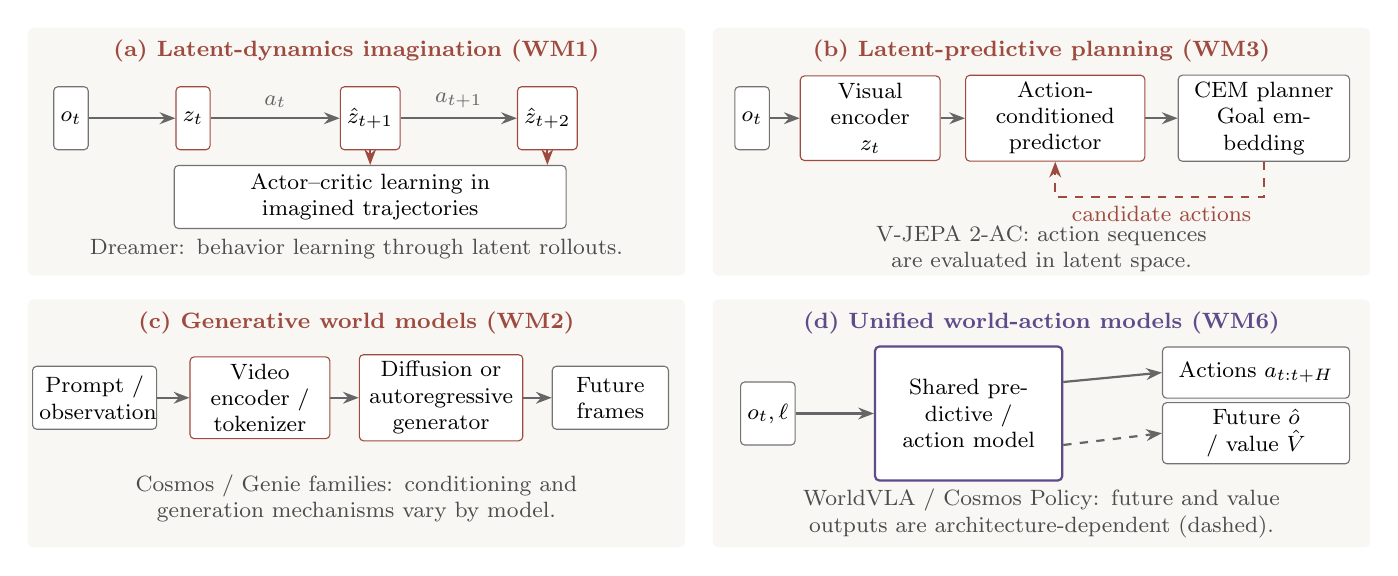
\begin{tikzpicture}[font=\figfont]
\tikzset{box/.style={fnode,minimum height=8mm},
 title/.style={font=\figfont\bfseries,align=center},
 note/.style={font=\figfont,align=center,text=black!70,text width=75mm}}
\foreach \x/\y in {0/0,8.7/0,0/-3.45,8.7/-3.45}{
 \fill[cPale!55,rounded corners=2pt] (\x,\y-2.1) rectangle +(8.35,3.15);}
\begin{scope}
\node[title,cWM] at (4.175,.75) {(a) Latent-dynamics imagination (WM1)};
\node[box,fill=white] (o) at (.55,-.1) {$o_t$};
\node[box,draw=cWM] (z0) at (2.1,-.1) {$z_t$};
\node[box,draw=cWM] (z1) at (4.35,-.1) {$\hat{z}_{t+1}$};
\node[box,draw=cWM] (z2) at (6.6,-.1) {$\hat{z}_{t+2}$};
\draw[farr] (o)--(z0);
\draw[farr] (z0)--node[above]{$a_t$}(z1);
\draw[farr] (z1)--node[above]{$a_{t+1}$}(z2);
\node[box,fill=white,text width=48mm] (ac) at (4.35,-1.1) {Actor--critic learning in imagined trajectories};
\draw[farr,cWM] (z1.south)--(ac.north);
\draw[farr,cWM] (z2.south)--(z2|-ac.north);
\node[note] at (4.175,-1.76) {Dreamer: behavior learning through latent rollouts.};
\end{scope}
\begin{scope}[xshift=8.7cm]
\node[title,cWM] at (4.175,.75) {(b) Latent-predictive planning (WM3)};
\node[box,fill=white] (o) at (.5,-.1) {$o_t$};
\node[box,draw=cWM,text width=16mm] (enc) at (2,-.1) {Visual encoder\\$z_t$};
\node[box,draw=cWM,text width=21mm] (pred) at (4.35,-.1) {Action-conditioned predictor};
\node[box,text width=20mm] (plan) at (7,-.1) {CEM planner\\Goal embedding};
\draw[farr] (o)--(enc);\draw[farr] (enc)--(pred);\draw[farr] (pred)--(plan);
\draw[farr,cWM,dashed] (plan.south)--(7,-1.1)--(4.35,-1.1)--(pred.south);
\node[inner sep=1.5pt,text=cWM] at (5.7,-1.32) {candidate actions};
\node[note] at (4.175,-1.76) {V-JEPA 2-AC: action sequences are evaluated in latent space.};
\end{scope}
\begin{scope}[yshift=-3.45cm]
\node[title,cWM] at (4.175,.75) {(c) Generative world models (WM2)};
\node[box,text width=14mm] (o) at (.85,-.2) {Prompt /\\observation};
\node[box,draw=cWM,text width=16mm] (enc) at (2.95,-.2) {Video encoder / tokenizer};
\node[box,draw=cWM,text width=19mm] (gen) at (5.25,-.2) {Diffusion or autoregressive generator};
\node[box,text width=13mm] (f) at (7.4,-.2) {Future frames};
\draw[farr] (o)--(enc);\draw[farr] (enc)--(gen);\draw[farr] (gen)--(f);
\node[note] at (4.175,-1.48) {Cosmos / Genie families: conditioning and generation mechanisms vary by model.};
\end{scope}
\begin{scope}[xshift=8.7cm,yshift=-3.45cm]
\node[title,cCONV] at (4.175,.75) {(d) Unified world-action models (WM6)};
\node[box] (o) at (.7,-.4) {$o_t,\ell$};
\node[box,draw=cCONV,thick,text width=22mm,minimum height=17mm] (m) at (3.25,-.4) {Shared predictive / action model};
\node[box,text width=22mm,minimum height=6.5mm] (a) at (6.9,.12) {Actions $a_{t:t+H}$};
\node[box,text width=22mm,minimum height=6.5mm] (f) at (6.9,-.65) {Future $\hat{o}$ / value $\hat{V}$};
\draw[farr] (o)--(m);
\draw[farr] ([yshift=4mm]m.east)--(a.west);
\draw[farr,dashed] ([yshift=-4mm]m.east)--(f.west);
\node[note] at (4.175,-1.67) {WorldVLA / Cosmos Policy: future and value outputs are architecture-dependent (dashed).};
\end{scope}
\end{tikzpicture}
\end{document}
